\section{Overall description}
\subsection{Product perspective}
	\subsubsection{System interfaces}\label{sec:systemInterfaces}
		The system we are to develop will have some external interfaces (represented in Figure \ref{fig:systemInterfaces}) to accomplish the goals stated in section 1.3.1\todo{reference?}.
		\begin{figure}[h]
			\centering
			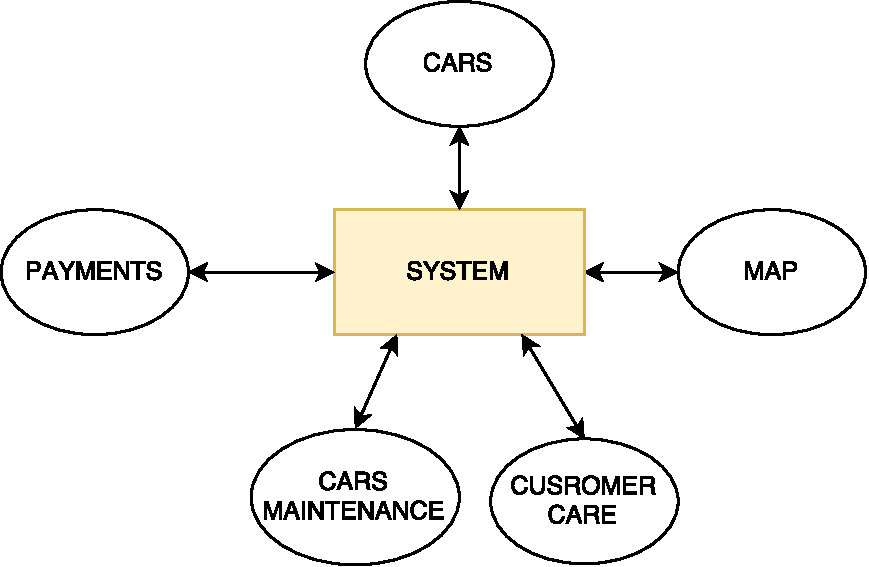
\includegraphics[scale=0.5]{system_blocks}
			\caption{
				\label{fig:systemInterfaces} 
				Overview of system interfaces
			}
		\end{figure}
	\paragraph{Payments}
	When a payment is required (e.g. when a user ends his rent) a request with all the details needed to complete the payment (i.d. name and surname of the user, due amount, credit card number etc.) is sent to an external payments system. Once the external system has completed the payment, it gives to our system a feedback of the payment process status so that we can take appropriate action.
	
	\paragraph{Customer care} Every time it is required a customer care service operator can contact a user. Customer care service operators can request and view all user details, their rent and payments history. Such operators can also ban or unban users from using the system, mark cars as not available and, in general, provide assistance to users during the rent.

	\paragraph{Maintenance} Every time maintenance for a car is required an external pool of maintenance operators is notified with GPS position of the car and a brief description of the problem.

	\paragraph{Map} GPS positions from cars and safe areas are displayed to all users, customer care operators and maintenance operators on a constantly updated map using an external reliable Geographic Information System.

%	\paragraph{Car} All cars have an integrated GPS system that continuously provides its position to our system-to-be. 
	
	
	
\subsubsection{User interfaces}\todo{where should user interface be mentioned? complete this}
	There are two main user interfaces: what we call here "application" and the car.\\
	Using the application users can:
	\begin{enumerate}
		\item Register and log-in to the system
		\item On the map they can view the position of
			\begin{enumerate}[label=\alph*)]
				\item themselves
				\item safe areas
				\item available cars (with their current battery level)
				\item charging stations
			\end{enumerate}
		\item Ask the customer care service for assistance 
	\end{enumerate}
	Using the interface in the car users can:
	\begin{enumerate}
		\item Start the engine
		\item View the real time battery level
		\item View their real time GPS position
		\item View their position w.r.t safe areas
		\item Terminate the rent\todo{through an interface? Must be so by definition!}
		\item Ask the customer care service for assistance
	\end{enumerate}			


	\todo{is this the right place?}In order to use all feature of our system a user must be registered. All guest users can register to our system providing some relevant information about themselves (such as name, surname, phone number, driving license, payment details etc.). A registered user can reserve one\todo{Only one at a time! Check reqs} available car for 1 hour, in this period of time he can reach the car he reserved and once he is nearby...

\subsubsection{Hardware interfaces}
	\todo{System must be able to talk back to cars(e.g. for position wrt safe areas)}All cars have an integrated GPS module that continuously provides its position to our system.

\subsubsection{Software interfaces}
	Databases and DBMSs are clearly required in order to store data about users, cars, charging stations, safe areas etc.
	As mentioned before (see Section \ref{sec:systemInterfaces}) the system need to use external APIs and to expose interfaces in order to interact with other systems.
	
\subsection{Domain assumption}
	We assume that these assumptions hold true in the domain of our system 
	\begin{itemize}
		\item GPS position is supposed to be accurate w.r.t. the defined areas
		\item GPS position and status of all cars is always available
		\item The user who reserves the car, will always be the person who drives it
		\item Users are legally allowed to drive cars (i.d. users have a proper driving license)
		\item Charging stations are always working and continuously monitored by the system
		\item Every time a user enters a car he ignites the engine
		\item All the data provided by users is correct and reliable
		\item 
	\end{itemize}